\section{Programmbeschreibung}\label{programm}

% Problemstellung/Fragestellung:
Die Anwendungssoftware „Flower Segmentation Tool“ wurde zur Erkennung von Arnica montana durch die Auswertung von Drohnenluftbildern entwickelt. Ziel ist es das Monitoring von Arnica montana durch eine nachhaltige Pflückung auf bisher nicht genutzte Flächen auszuweiten. Durch den Drohneneinsatz können auch in unwegsamen Gelände Erkenntnisse über den Bestand von Arnika gewonnen werden. Als Datengrundlage bei der Entwicklung dienten die Aufnahmen der Testflüge aus dem Schwarzwald des „Projekt zum Schutz der Biodiversität in Rumänien“.
Das „Flower Segmentation Tool“ ist so konzipiert, dass schnelle Berechnungen Aussagen über den Bestand getroffen werden können, die dann vor Ort weiter untersucht werden. Es soll also unterstützend zur Feldarbeit wirken und dabei eine Einschätzung liefern, wo diese stattfinden kann.
%Anforderungen an den Code
Die wichtigste Anforderung an das Programm ist dabei trotz großer Datenmengen noch in angemessener Schnelligkeit zu agieren. Um eine einfache Installation zu ermöglichen, wurde darauf geachtet niedrigschwellige Soft- und Hardwarevoraussetzungen zu fordern. 
%Anforderungen an die Benutzeroberfläche

\begin{figure}[hbt]
 \centering
 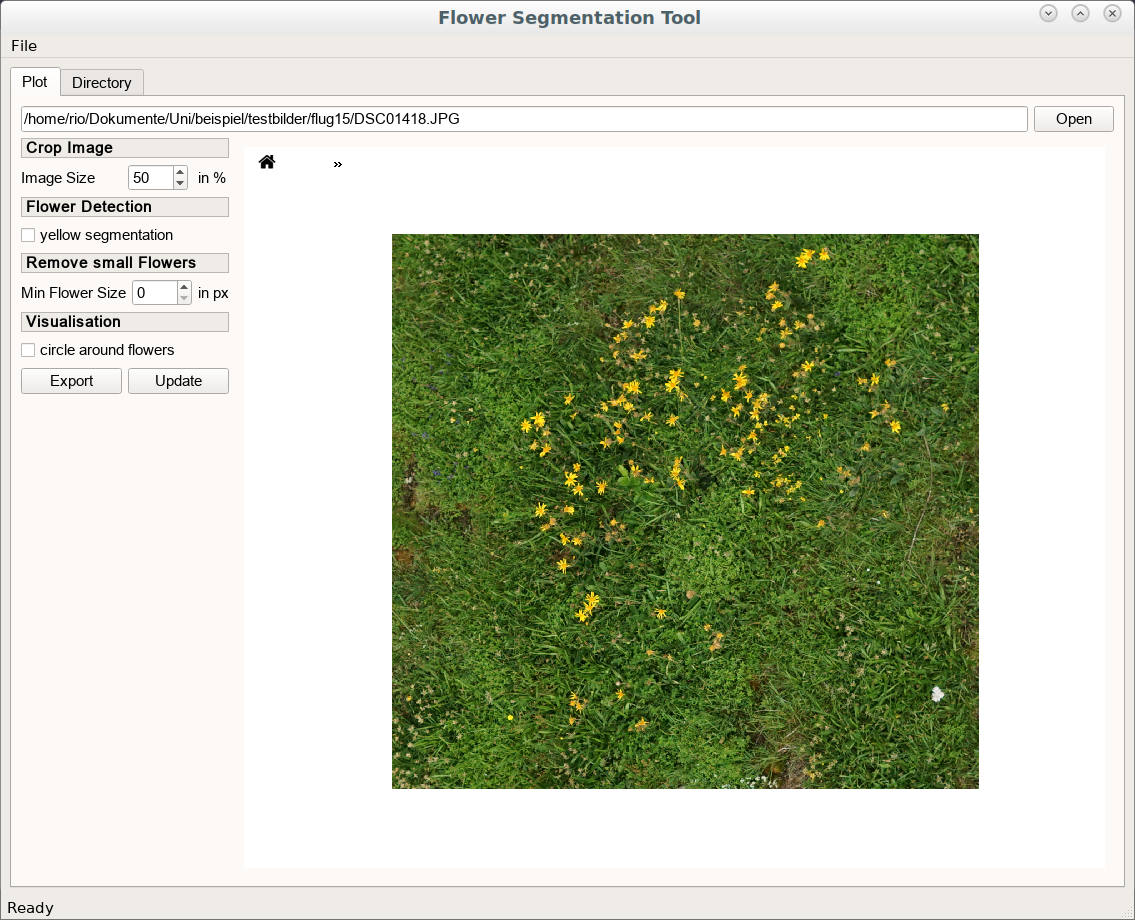
\includegraphics[width=\textwidth,angle=0]{abb/gui/plot-fenster-mit}
 \caption{Grafische Oberfläche mit Plotfenster}
\label{fig:gui-plot}
\end{figure}

Die Grafische Benutzeroberfläche besteht aus zwei Teilen. Einerseits soll die grafische Darstellung der Bilder zum Ausprobieren der Parameter möglich sein (Siehe Abbildung~\ref{fig:gui-plot}, S.~\pageref{fig:gui-plot}). Dabei ist ein vielseitiger Plotfenster mit der Möglichkeit den Ausschnitt zu verändern und Teile des Bildes zu vergrößern eine wichtige Funktion. Andererseits soll eine einfache Anwendung der Berechnung auf einen großen Datensatz möglich sein. Deshalb gibt es unter dem Tab „Directory“ die Eingabe oder Auswahl eines Ordners (Input-Directory), aus dem alle Bilddateien bearbeitet werden (Siehe Abbildung~\ref{fig:gui-dir}, S.~\pageref{fig:gui-dir}). Bei beiden Tabs verschafft eine Statusanzeige im unteren Rand des Anwendungsfensters einen Überblick, welche Prozesse im Hintergrund laufen.

\begin{figure}[htb]
 \centering
 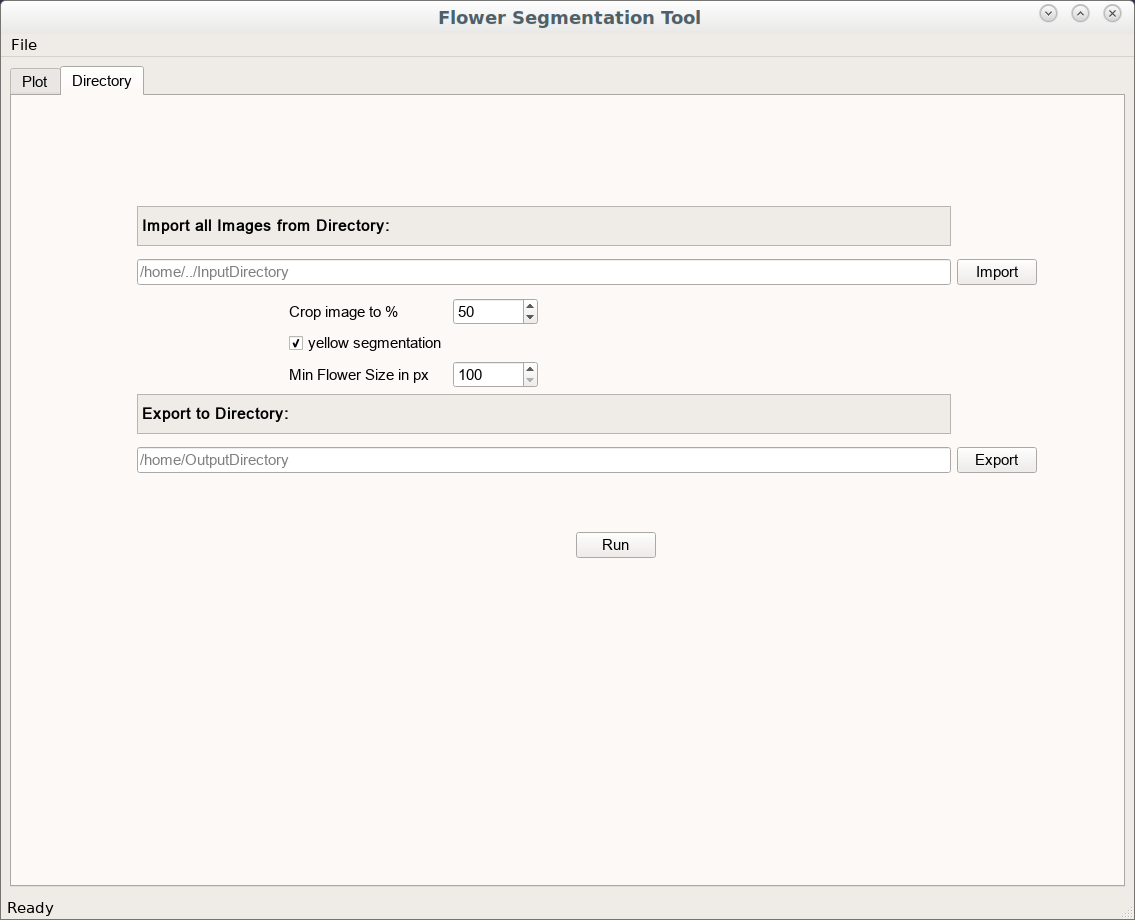
\includegraphics[width=\textwidth,angle=0]{abb/gui/directory-fenster}
 \caption{Grafische Oberfläche zur Anwendung auf Ordner}
\label{fig:gui-dir}
\end{figure}

\subsection{Programmiersprache}
Python ist eine Open Source Programmiersprache, die plattformübergreifend auf allen gängigen Betriebssystemen anwendbar ist. Die interpretierte Skriptsprache wurde 1994 von dem niederländischen Programmierer Guido Rossum als Python 1.0 veröffentlicht. Der Name Python hat Rossum von der britischen Komikergruppe Monty Python abgeleitet.
Entscheidener Unterschied zu anderen höheren Programmiersprachen, ist der gut lesbare und knapp gehaltene Stil von Python. Ziel ist es Redundanz zu vermeiden und Übersichtlichkeit zu optimieren. Zur Strukturierung verwendet Python Einrückungen und kommt mit wenigen Schlüsselwörtern aus. Mit diesem reduzierten Syntax schafft Python Einfachheit, ohne dabei eine Komplexität zu verhindern. Python unterstützt objektorientierte und funktionale Programmierung. Es gibt eine umfassende  Standartbibliothek und zusätzlich die Möglichkeit der Erweiterung einer Vielzahl an Modulen, die in den Skripten importiert werden können.
%Vielzahl von NutzerInnen (kommerziell, wissenschaftlich, Betriebssystemen, Webframeworks)
%- Python-Interpreter, die stärksten sind CPython, basiert auf der Programmiersprache C und Jython basierend auf Java. Compiler, die Python in andere Programmiersprachen übersetzten und dort nutzbar machen.

Seit 2001 wird Python durch die Python Software Foundation stetig weiterentwickelt. Python 2 gibt es seit 2000, Python 3 seit 2008. Dies beinhaltet so tiefgreifende Änderungen, dass einige Funktionen, die unter Python 2 geschrieben wurden, nicht mehr unter Python 3 funktionieren würden. Deshalb wird Python 2.7 noch bis Ende 2019 mit weiteren Updates unterstützt. Die aktuellste stabile Version ist seit 2018 Python 3.7 \citep[vgl.][]{PSF2019}.

%Verweis auf Einstiegsmöglichkeit in die verwendete Programmiersprache-> Anhang

%Verwendete Pakete???
\subsection{Anwendungsbereich} %Zusammenfassung Anwendungsmöglichkeiten des Programms
Das Programm zur automatischen Erkennung von Arnika soll zur Bildanalyse und Auswertung von Luftaufnahmen, die von Drohne aufgenommen wurden, angewendet werden. Es können RGB Fotos eingelesen und analysiert werden. Bei der Erfassung einer Fläche mit einer Drohne werden die Bilder so aufgenommen, dass es immer eine große Überlappung gibt. Dies ist notwendig, damit auch sichergestellt werden kann, dass die gesamte Fläche erfasst ist. Das Programm kann diese Überlappung manuell durch Zuschnitt auf die Mitte des Bildes verringern. Von den RGB Bildern kann dann durch Segmentierung allein der gelbe Farbbereich angezeigt werden. Die Anzeige kann auf eine Mindestgröße für zusammenhängenden gelbe Farbpixel eingestellt werden, damit deutlich kleinere Blumen heraus gefiltert werden können. Eine weitere Möglichkeit der visuellen Darstellung ist die Umrandung von gefundenen zusammenhängenden Komponenten (Connected Components, kurz: CC) im ursprünglichen Bildausschnitt. Auch dabei lässt sich die Mindestgröße wieder manuell festlegen. So können verschiedene Parameter ausprobiert, im Plotfenster dargestellt und angepasst werden. Hierbei ist die Navigationsleiste des Plotfenster sehr hilfreich, die verschiedene Zoom und Anzeigefunktionen besitzt. Die Berechnung und Darstellung des einzelnen Bildes kann dann exportiert werden. Um einen gesamten Datensatz einer Drohnenbefliegung bearbeiten zu können, lassen sich Berechnungen mit gewählten Parametern auch auf alle Bilder eines Ordners anwenden.  

% Einordnung in die "Aufgabe des Programms" für das Projekt???
%genaue Funktionen (zentrierter Crop, Bilder plotten lassen, exportieren, segmentieren, circles, dabei größe anpassen)
\subsection{Programmaufbau}

Der Programmaufbau des Flower Segmentation Tools ist als Python Programmpaket strukturiert. Es kann deshalb auch mit pip aus dem Python Package Index (PyPI) heruntergeladen und installiert werden. In Abbildung \ref{fig:folders} auf S. \pageref{fig:folders} ist die Ordnerstruktur dargestellt. Das Paket befindet sich im Ordner \texttt{segmentationtool}, welches aus mehreren Unterpaketen besteht. Im Paket \texttt{filter} befindet sich das \texttt{data.py} Modul mit der \texttt{Data class}. Im Ordner \texttt{gui} sind alle Pakete und Module, die die Grafische Benutzeroberfläche (grafical user interface, kurz: GUI) bilden. Dazu gehört auch das \texttt{pyqt5backend} das mit dem Programm Qt5Designer erstellt wurde. Mit der Datei \texttt{main.py} kann das Programm mit der GUI aufgerufen werden. 

test, build, Readme license setup


\begin{figure}[H]
\footnotesize
  \begin{forest}
    pic dir tree,
    where level=0{}{
      directory,
    },
    [segmentationtool
      [dist
      ]
      [build
      ]
      [filter
        [\textunderscore \textunderscore init\textunderscore \textunderscore .py, file
        ]
        [data.py, file
        ]
      ]
      [gui
        [pyqt5backend
          [\textunderscore \textunderscore init\textunderscore \textunderscore .py, file
          ]
          [guidesign.py, file
          ]
          [mplwidget\textunderscore nav.py, file
          ]
          [new.ui, file
          ]
        ]
        [\textunderscore \textunderscore init\textunderscore \textunderscore .py, file
        ]
        [app.py, file
        ]
      ]
      [tests
      ]
      [images
        [testimages
        ]
        [output
        ]
      ]
      [main.py, file
      ]
      [setup.py, file
      ]
      [README.md, file
      ]
      [LICENSE, file
      ]
    ] 
  \end{forest}
  \caption{Ordnerstruktur}
  \label{fig:folders}
\end{figure}

Die inneren Prozesse einer Plotabfrage werden in Abbildung \ref{fig:flowchart} (S. \pageref{fig:flowchart}) in einer Flowchart, auch Programmablaufplan genannt, dargestellt. Bei der Aktualisierung des dargestellten Bildes mit veränderten Parametern ist die Codestruktur so angelegt, dass möglichst keine Wiederholung unnötiger Berechnungen stattfindet. Hauptintention dabei stellt die Minimierung von Zeitverzögerungen da. Mit der Verwendung von if-else Schleifen werden je nach Prozess der berechnet wird zunächst erstmal abgefragt, ob sich die Parameter überhaupt verändert haben. Ist dies nicht oder nur teilweise der Fall kann eine erneute komplette Berechung nicht notwenig sein und der angefragte Prozess auf ein schon gespeichertes Bild oder eine Teilfunktion direkt zurückgreifen kann. 

Bei der Darstellung der Elemente eines Programmablaufplans ist nach ihrer Funktion in der Programmabfrage kategorisiert. Die Start- oder Stop-Elemente sind als gelbe Rechtecke mit gerundeten Ecken gekenntzeichnet. Ein Parallelogramm symbolisiert eine Ein- oder Ausgabe. In diesem Fall nur Ausgabe, die auch gleichzeitig das Ende der Abfrage bedeutet und daher hier in der selben Farbe, wie die Startelemente dargestellt. Die Rechtecke zeigen eine Tätigkeit oder Operation, in diesem Fall Methoden der Data Klasse, an. Entscheidungen werden als Rauten dargestellt, dessen Abfrage mit „Ja” beantwortet immer nach unten weiter verläuft.
Die \texttt{initial plot} Abfrage wird nach dem ersten Öffnen des Bildes aufgerufen. Das Bild wird als Objekt der Data class instanziiert und kann als (\texttt{self.img}) abgerufen werden. 



Der Aufruf des Gesamtfilters, der die gelben Bildteile mit einer Mindestgröße segmentiert, ruft Funktionen auf, die jeweils auch direkt von anderen Anfragen angesprochen werden können. Dabei werden die Zwischenergebnisse als Objekte der Klasse gespeichert. Insgesamt kann so die Ausgabe effizienter und schneller wiedergegeben werden, gerade bei Bilder, die eine große Datenmenge einnehmen.

%- cb erklären, Symbole erklären, Detailiert den Verlauf der Abfrage erklären. 

\begin{figure}[htb]
 \centering
 \includegraphics[width=\textwidth,angle=0]{abb/programm/prozesse}
 \caption{Programmablaufplan der Plotabfrage}
\label{fig:flowchart}
\end{figure}

\subsection{Vorgehensweise Methoden?}

genaue Beschreibung der Methoden (Wie wird der Bereich heraus gefiltert, Datenstruktur?, GUI, Parameter)
nach welchen Kriterien und warum diese gewählt -> Quellen?

Methoden: 
- Filtern nach Farbebereich ->
Allen Bildpunkten, die nicht in dem Farbbereich zwischen RGB (200, 133, 0) und (255, 255, 122) liegen, wird mit der Hilfe einer Maske 0 zugeordnert. 

- 

% dafür wird das Bild als dreidimensioneller BGR-Array mit je einer Ebene je Farbband. Mit der Funktion cv2.inRange() wird eine Maske erstellt, die für alle Pixel, die nicht in dem Bereich sind 0 zuordnet und für alle die in dem Bereich sind 255. Diese Maske lässt sich auf das originale Bild mit cv2.bitwise() übertragen. Dabei werden zwei Bilder zusammengefügt, im Bereich einer Maske.??doppelt?? 
Warum nach Farbbereich filter:
strong argument -> Starkes Charakteristika der Arnika Blume ist die Farbe. Dies als erstes Erkennungsmerkmal gewählt.


Datenstruktur:
Dazu einleitung: Objektorientierte Programmierung, vorteile?
- Inheritence (Vererbung)
- Composition (Aufbau)
Multiple instances
Customization via inheritance
Operator overloading
Es gibt die Data class, die ein Bild als Instanz lädt und deren Objekte die durch Methoden veränderte Bilder sind. 
DesignerMainWindow class als gesamt GUI, die dann alle anderen Dinge "erbt" bzw. aufruft.
Es gibt das MplWidget als class, die die Canvas class aufruft und das Plotfenster bildet und Teil der Gui ist. 
Gui mit pyqt5 Backend geschrieben und mit dem Qt5Designer erstellt.



\subsubsection{Parameterbeschreibung}
Der Percent parameter geht immer vom original bild aus und schneidet es auf die gewünschte Prozentzahl mittig zu. Bei änderung, wird wieder auf das original bild referenziert

Min Size in pixel: 

\subsection{Implementierung / Aufruf}    


% Flow-Chart für die GUI und den Programmaufruf, quasi als "Anleitung der Benutzung"

% Beschreibung der genauen Eingabe, wie im ersten Abschnitt mit den Gui-screenshots schon angefangen. 

%Navigationtoolbar beschreiben: 
%https://github.com/matplotlib/matplotlib/blob/master/doc/users/navigation_toolbar.rst


\subsubsection{Hard- und Softwarevoraussetzungen}

Python 3 

\subsubsection{(Notwendige) In- und Output-Dateien und deren Formate}


- Einbindungsmöglichkeiten in andere Anwendungen
- Bei komplexen Berechnungsverfahren Beschreibung der Algorithmen und Literaturhinweise zu den Quellen der Verfahren


    
